다음 그림의 $\square\mathrm{ABCD}$에서 $\overline{\mathrm{AE}} = \overline{\mathrm{EF}} = \overline{\mathrm{FD}}$, $\overline{\mathrm{BG}} = \overline{\mathrm{GH}} = \overline{\mathrm{HC}}$일 때, $\square\mathrm{EGHF} = k \square\mathrm{ABCD}$를 만족시키는 상수 $k$의 값을 구하여라.

\begin{figure}[h]
\centering
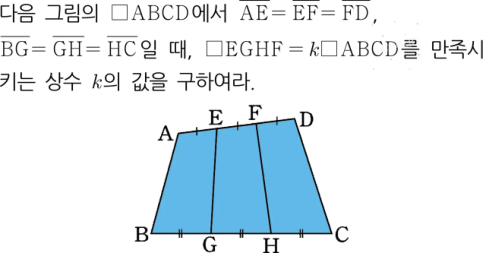
\includegraphics[width=0.4\textwidth]{_OUTPUT_/area_problem_01_figure.png}
\end{figure}
